\subsection{Communication Serveur - Drone}

\begin{figure}[ht]
\begin{center}
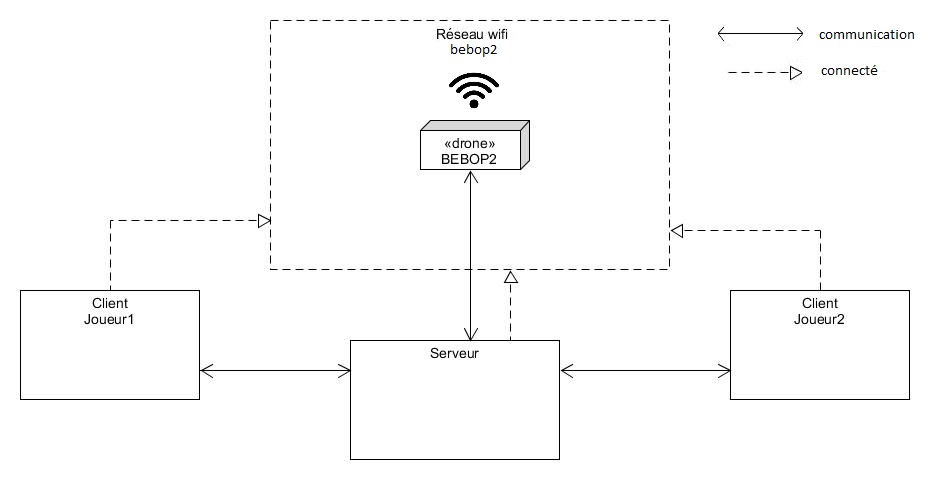
\includegraphics[scale=0.45]{images/architecture.jpg}
\caption{Schéma de communication entre les différents appareils}
\end{center}
\end{figure}

La partie communication entre le serveur et le drone est le point le plus délicat du projet et se trouve au c\oe{}ur de notre problématique. En effet, on rappelle que l'objectif principal est le pilotage du drone par un programme \og fait maison \fg{}. Contrairement à la communication entre les clients mobiles et le serveur, aucun protocole n'a dû être spécifiée manuellement puisque nous nous sommes servis des outils de développement mis à disposition par le constructeur pour les développeurs. En effet, comme expliqué plus loin dans la section \ref{impl} l'utilisation des primitives C ont permis d'établir la connexion avec le drone et de lui envoyer des commandes de déplacement avec un certain niveau d'approche bien qu'il ne soit pas très élevé sans pour autant être trop compliqué d'un point de vue mécanique. Les déplacements sont gérés par un jeu d'instructions qui influencent l'inclinaison de l'appareil et la vitesse de rotation du lacet\footnote{En aéronautique, désigne le mouvement de rotation horizontal du mobile autour d'un axe vertical}. 

Plusieurs tests et observations ont été nécessaires pour connaître les effets des différentes instructions sur les mouvements du drone ce qui a rendu cette étape relativement difficile. À cela viennent s'ajouter des conditions de travail non optimales à savoir une disponibilité limitée du drone pour effectuer des tests ainsi qu'un environnement de tests non idéal pour prévenir des dommages sur l'appareil qui sont inévitables.

Par exemple, plusieurs hélices ont été endommagées au point qu'il nous a fallu en commander ou quelques blessures dues à une mauvaise manipulation ont été provoquées. L'autonomie relativement limitées constituait elle aussi un obstacle dans les tests qui se retrouvaient ainsi prématurément suspendus.

